\documentclass[10pt,letterpaper]{article}
\usepackage[top=0.85in,left=1.75in,footskip=0.75in,marginparwidth=1in]{geometry}

% use Unicode characters - try changing the option if you run into troubles with special characters (e.g. umlauts)
\usepackage[utf8x]{inputenc}
\usepackage{textgreek}
\usepackage[scaled]{helvet}
\usepackage[T1]{fontenc}
\renewcommand\familydefault{\sfdefault}

% file names with period in name, without using braces {}.pdf
\usepackage{grffile}

% clean citationshttps://www.overleaf.com/project/60d45824b01a0838903d992f
\usepackage{cite}

% clean math
\usepackage{amsfonts}
% \usepackage{amsmath,amssymb,amsfonts}
\usepackage{mathtools}

\usepackage[separate-uncertainty=true, multi-part-units=single]{siunitx}
\newcommand{\micron}{\micro\meter}
\newcommand{\fL}{\femto\liter}
\newcommand{\mmol}{\milli\mol}
\newcommand{\photons}{\micro\mol\per\square\meter\per\second}
\newcommand{\ugml}{\micro\gram\per\milli\liter}
\newcommand{\M}{\textsc{M}}%\mole\per\litre}
\newcommand{\uM}{\micro\textsc{M}}%\mole\per\litre}
\newcommand{\gcdw}{\gram_\text{\tiny DCW}}
\newcommand{\cmol}{\textsc{C$\cdot$}\mol}
\newcommand{\cellvolume}{\milli\liter_\text{\tiny cell}}
\sisetup{range-phrase = \text{--}}

\newcommand{\mL}{\milli\liter}
\newcommand{\gpl}{\gram\per\liter}
\newcommand{\mM}{\milli\textsc{M}}%\mole\per\liter}
\newcommand{\ngpul}{\nano\gram\per\micro\liter}

\newcommand{\cuparrow}{\textcolor{blue}{$\pmb\uparrow$}}
\newcommand{\cdoarrow}{\textcolor{red}{$\pmb\downarrow$}}

\newcommand{\cqgel}{\ensuremath{C_{\text{gel}}}}
\newcommand{\cqtop}{\ensuremath{C_{\text{topoI}}}}



% nice:
%\usepackage{markdown}

% hyperref makes references clicky. use \url{www.example.com} or \href{www.example.com}{description} to add a clicky url
\usepackage{nameref,hyperref}

% line numbers
\usepackage[right]{lineno}

% improves typesetting in LaTeX
\usepackage{microtype}
\DisableLigatures[f]{encoding = *, family = * }

% text layout - change as needed
\raggedright
\setlength{\parindent}{0.5cm}
\textwidth 6.25in 
\textheight 8.75in

% Remove % for double line spacing
%\usepackage{setspace} 
%\doublespacing

% use adjustwidth environment to exceed text width (see examples in text)
\usepackage{changepage}

% adjust caption style
\usepackage[aboveskip=1pt,labelfont=bf,labelsep=period,singlelinecheck=off]{caption}

% remove brackets from references
\makeatletter
\renewcommand{\@biblabel}[1]{\quad#1.}
\makeatother

% headrule, footrule and page numbers
\usepackage{lastpage,fancyhdr,graphicx}
\usepackage{epstopdf}
\pagestyle{myheadings}
\pagestyle{fancy}

% no section numbers
\setcounter{secnumdepth}{0}

\fancyhf{}
\rfoot{\thepage/\pageref{LastPage}}
\renewcommand{\footrule}{\hrule height 2pt \vspace{2mm}}
\fancyheadoffset[L]{2.25in}
\fancyfootoffset[L]{2.25in}

% use \textcolor{color}{text} for colored text (e.g. highlight to-do areas)
\usepackage{xcolor}


% this is required to include graphics
\usepackage{graphicx}

% use if you want to put caption to the side of the figure - see example in text
\usepackage{sidecap}

% use for have text wrap around figures
\usepackage{wrapfig}
\usepackage[pscoord]{eso-pic}
\usepackage[fulladjust]{marginnote}
\reversemarginpar

% define custom colors (this one is for figure captions)
\definecolor{Gray}{gray}{.25}
\definecolor{lgold}{RGB}{255, 215, 10}

% MAKROS
\newcommand{\scyst}{\textit{Synechocystis} PCC6803}
\newcommand{\scst}{\textit{Synechocystis}}

\newcommand{\gene}[1]{\ensuremath{\textit{#1}}}
\newcommand{\gyra}{\gene{gyrA}}
\newcommand{\gyrb}{\gene{gyrB}}
\newcommand{\topa}{\gene{topA}}

\newcommand{\gyrkd}{\ensuremath{\text{gyr}^{\text{KD}}}}
\newcommand{\gyrakd}{\ensuremath{\text{gyrA}^{\text{KD}}}}
\newcommand{\gyrbkd}{\ensuremath{\text{gyrB}^{\text{KD}}}}
\newcommand{\gyrabkd}{\ensuremath{\text{gyrAB}^{\text{KD}}}}
\newcommand{\topakd}{\ensuremath{\text{topA}^{\text{KD}}}}
\newcommand{\topaox}{\ensuremath{\text{topA}^{\text{OX}}}}

\newcommand{\OD}{\ensuremath{\text{OD}_{750}}}
\newcommand{\dOD}{\ensuremath{\text{OD}_{\lambda}}}
\newcommand{\ox}{\ensuremath{\text{O$_2$}}}
\newcommand{\cox}{\ensuremath{\text{CO$_2$}}}

% EDITING: rm for publication
\usepackage{todonotes}
\newcommand{\raim}[1]{\begingroup{\color{purple}#1}\endgroup}
\newcommand{\ilka}[1]{\begingroup{\color{blue}#1}\endgroup}
\newcommand{\selma}[1]{\begingroup{\color{red}Salima: #1}\endgroup}
\newcommand{\TODO}[1]{\begingroup\color{red}*** #1 ***\endgroup}

\newcommand{\remove}[1]{\begingroup\color{gray}\endgroup}
\newcommand{\cut}[1]{\begingroup\color{gray}#1\endgroup}


% document begins here
\begin{document}
\vspace*{0.35in}

% title goes here:
\begin{flushleft}
{\Large Plasmid Supercoiling is low During the Dark Phase in
  Cyanobacteria: A Clarification of the Interpretation of
  Chloroquine-Supplemented Agarose Gels}

Salima R\"udiger\textsuperscript{1}, 
Anne Rediger, Adrian K\"olsch\textsuperscript{4}, Dennis Dienst,
Ilka M. Axmann\textsuperscript{1,*},
Rainer Machn\'e\textsuperscript{1,2,*},
\\
\bigskip
\bf{1} Institut f. Synthetische Mikrobiologie, Heinrich-Heine Universit\"at, D-40225 D\"usseldorf, Germany
\\
\bf{2} Institut f. Quantitative u. Theoretische Biologie, Heinrich-Heine Universit\"at, D-40225 D\"usseldorf, Germany
\\
\bf{4} Physics Department, Freie Universität Berlin, D-14195 Berlin, Germany
%Freie Universität Berlin, Physics Department, Arnimallee 14, 14195 Berlin, Germany
\bigskip
* machne@hhu.de (RM) and axmann@hhu.de (IMA)

\end{flushleft}

\section*{Abstract}
In cyanobacteria DNA supercoiling varies over the diurnal light/dark
cycle and is integrated with the temporal transcription and
replication programs. Woelfe \textit{et al.} (2007, PNAS) have
reported that DNA supercoiling of an endogenous plasmid was
progressively higher during prolonged dark phases in
\textit{Synechococcus elongatus} PCC 7942.  This is counterintuitive,
since higher levels of negative DNA supercoiling are commonly
associated with exponential growth and high metabolic flux. Vijayan
\textit{et al.} (2009, PNAS) then have silently reverted the
interpretation of plasmid mobility on agarose gels supplemented with
chloroquine (CQ), but not further discussed the differences.
%
Here, we set out to clarify this open issue in cyanbacterial DNA
supercoiling dynamics. We first re-capitulate Keller's band counting
method (1975, PNAS) using CQ instead of ethidium bromide as the
intercalating agent.  A 500x--1000x higher CQ concentration is
required in the topoisomerase I reaction than in the agarose gel
buffer to achieve full plasmid relaxation. This is likely due to the
dependence of both, the DNA binding affinity and the DNA unwinding
angle, on the ionic strength of the buffer. We observe that lower
levels of CQ are required to fully relax \textit{in vivo} pUC19
supercoiling than was used by Woelfle \textit{et al.}. Next we
analyzed the \textit{in vivo} supercoiling of endogenous plasmids of
\textit{Synechococcus elongatus} and \textit{Synechocystis sp.} PCC
6803, at two different CQ concentrations.  This clearly indicates that
negative supercoiling of plasmids does not increase but decreases in
the dark phase, and proressively decreases in prolonged dark.




% now start line numbers
\linenumbers


\section{Introduction}
\textit{In vivo}, the DNA double helix usually exists in a torsionally
strained state, often just denoted as negative DNA supercoiling.  The
energy stored in underwound DNA can be channeled locally at gene
promoters to open and ``read'' DNA in transcription and replication.
In Bacteria, the level of DNA supercoiling is homeostatically controlled by
enzymes but also depends on the transcription and replication, and
in turn influences transcription rate of many genes \cite{Dorman2019}. 
%
The genome-wide levels of DNA supercoiling are difficult to measure,
and often endogenous or transfected plasmids are used as a proxy
measurement for \textit{in vivo} supercoiling levels. Plasmids that
differ topologically (topoisomers) can be separated on agarose gels,
where each topoisomer forms a distinct band. Plasmids with a higher
level of negative or positive supercoiling are more compact and
migrate faster (further) on agarose gels. However, the dynamic range
of separable topoisomers is small, and the \textit{in vivo} level of
plasmid supercoiling leads just to broad (smeared) band that consist
of several topoisomers. Intercalating substances locally unwind DNA
and thereby can be used to quench supercoiling.  When adding the right
amount of such an intercalator, e.g. ethidium bromide or chloroquine,
plasmid supercoiling can be reduced to a level where topoisomers are
again separable in agarose gels. Increasing the amount of the intercalator
can further convert originally negatively supercoiled plasmids to
positively supercoiled plasmids.

Similarly, intercalators can be used together with a supercoil
relaxing enzyme such as bacterial topoisomerase I to generate a series
of plasmid samples with continuously less supercoiling. Keller
combined the use of an intercalator (ethidium bromide) at different
concentrations in such a relaxation series and on agarose gels. All
bands from the original state of the plasmid to the fully relaxed form
can then be counted to determine the so-called linking number deficit
($\Delta Lk$) of a plasmid sample. $\Delta Lk$ is the difference of the
number of crossing of the two helix strands aroud each other (the
linking number) in the supercoiled plasmid and the relaxed form, where
the helix has about \SIrange{10.4}{10.5}{bp} per helix turn.


Mori and Johnson first suggested that supercoiling could underlie the
regulation of hundreds of genes during the light/dark (diurnal) cycle
in cyanobacteria \cite{Mori2001}. Indeed, genome compaction varied
over the diurnal cycle \cite{Smith2006}. 

conflicting results and interpretations in two papers
\cite{Woelfle2007} vs. \cite{Vijayan2009},
hidden by a different formula to determine relative mobility $RM$:

\cite{Woelfle2007} evaluated their gel as:

\begin{equation}
  RM = (median - Rel)/(SC - Rel)
\end{equation}
upper band: Rel (O.C.!), lower band: SC,

while \cite{Vijayan2009} used: 
\begin{equation}
  RM = 1 - (mean - oc)/(oc - rel)
\end{equation}

upper band: oc (open circular), lower band: rel for relaxed,
unclear why oc and rel would travel differently,
inconsistent signs - likely $|oc-rel|=rel-oc$.
       
Direct comparison:

\begin{align}
  RM =& (target - upper)/lower - upper)\\
  RM =& 1 - (target - upper)/(upper - lower)
\end{align}




\section{Results}

\paragraph{Keller's Band Counting Method with Chloroquine.}
To establish the effect of chloroquine (CQ) on plasmids, we
recapitulated Keller's band counting method but using chloroquine
instead of ethidium bromide (EtBr) as the intercalating agent
(Fig. \ref{fig:keller}).
%
In Keller's protocol \cite{Keller1975b} the indicated EtBr
concentrations in the topoI reaction ranged from
\SIrange{0}{6.9}{\uM}. With a molecular mass of
\SI{394.3}{\gram\per\mol}, the highest concentration is
\SI{2.7}{\ugml}. In the gels the maximal concentration was
\SI{0.06}{\ugml}. That is, in the topoI reaction, up to 45x more EtBr
was used in the topoisomerase I relaxtion reactions than in the gels
to achieve the similar plasmid relaxation effects.

\TODO{gel buffers have high ionic strength, required for gel electrophoresis,}

\TODO{EtBr:DNA dissociation constant, dependence on ionic strength}

\TODO{more or less undwinding angle and lower or higher dissociation
  constant with ionic strength?\\ The unwinding angle for chloroquine
  increases with ionic strength \cite{Jones1980}, while it is
  independent for EtBr. The CQ:DNA dissociation constant, varied from
  \SIrange{27}{2600}{\uM}, depending on the ionic strength of the
  buffer \cite{KwakyeBerko1989}.}

\TODO{here 0.5xTBE for gel and, the CutSmart buffer for the topoI
  reactions}

Figure \ref{fig:keller} shows that the lowest CQ concentrations in the
gel ($\cqgel=\SI{1}{\ugml}$) was sufficient to detect a clear change
in the migration of the pUC19 topoisomers. The relaxed plasmids
($\cqtop=\SIrange{0}{200}{\ugml}$) had already shifted to positive
supercoiling and migrated faster than without CQ.  Topoisomers treated
with $\cqtop=\SIrange{800}{1000}{\ugml}$ were all close to full
relaxation. The untreated \textit{in vivo} sample (``C'') appeared
fully relaxed at $\cqgel=\SI{2}{\ugml}$, and shifted to positive
supercoiling at $\cqgel>\SI{4}{\ugml}$.



\begin{figure}[ht!]
    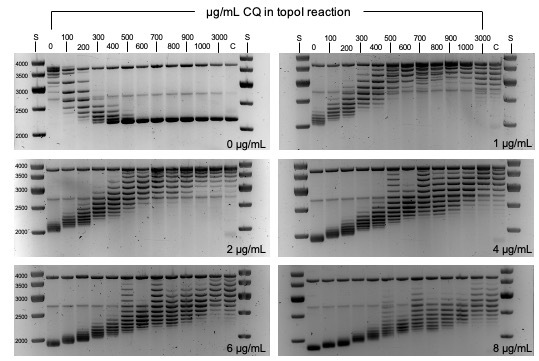
\includegraphics[width=\textwidth]{figures/keller_puc19.jpg}
  \caption{\textbf{pUC19 on 1.2 \% agarose gel supplemented with 0--8
      \si{\ugml} chloroquine.} Samples of the pUC19 plasmid, isolated
    from \textit{E. coli}, were treated with 0--3000 \si{\ugml}
    chloroquine and topoisomerase I as indicated (lanes). The sample
    “C” is untreated pUC19 as control. Size marker "S" is the
    GeneRuler 1 kb DNA Ladder. The samples were split an separated on
    6 agaose gels, each supplement with a chloroquine concentration
    from 0 to 8 \si{\ugml} as indicated (lower right). The top band
    in each gel is the open circular form. The band between  2.5 kb and 3 kb
    is the linear form of the plasmid.}
  \label{fig:keller} 
\end{figure}





\begin{figure}[ht!]
  \begin{minipage}{.49\textwidth}
    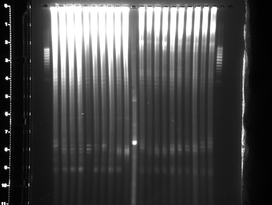
\includegraphics[width=\textwidth]{figures/diurnal/Y_CQ01_high_exposure.png}
  \end{minipage}
  \begin{minipage}{.49\textwidth}
    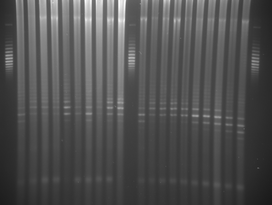
\includegraphics[width=\textwidth]{figures/diurnal/20130618_1511.png}
  \end{minipage}
  
  \vspace{-.5cm}
  \textbf{C}
  \vspace{.25cm}
  
  \begin{minipage}{.49\textwidth}
    
\includegraphics[width=\textwidth]{figures/diurnal/20130620_pCA_CQ1.png}
  \end{minipage}
  \begin{minipage}{.49\textwidth}
    
\includegraphics[width=\textwidth]{figures/diurnal/20130821_pCA_CQ20.png}
  \end{minipage}
  
  \vspace{-.5cm}
  \textbf{A}\hspace{.32\textwidth}\textbf{B}\hspace{.32\textwidth}\textbf{D}

  \caption{\textbf{Chloroquine Gel Analysis: Calibration \& Diurnal
      Supercoiling}. \small{\textbf{A \& B:} agarose gels of plasmid
      extracts from a diurnal growth experiments (see F); supplemented
      with \SI{1}{\ugml} (A) or \SI{20}{\ugml} (B) chloroquine
      diphosphate (CQ).  Additional lanes (left, right, center) show
      the pUC19 plasmid isolated from \textit{E.coli} cultures as a
      control, or (only A, central lane) a pooled plasmid sample after
      treatment with NcoI restriction enzyme which cuts only the
      pCA2.4\_M plasmid (one cut site) but not the similarly sized
      pCB2.4\_M. All topoisomer bands are replaced by a single band of
      linearized pCA2.4\_M. \textbf{C \& D:} Southern blots of the
      gels in (A) and (B) using probes specific for the pCA2.4\_M
      plasmid confirms the identity of the plasmid bands (Table
      \ref{tab:blot}).}}
    \label{fig:diurnalcq} 
\end{figure}


\begin{figure}
  \begin{minipage}{.27\textwidth}
    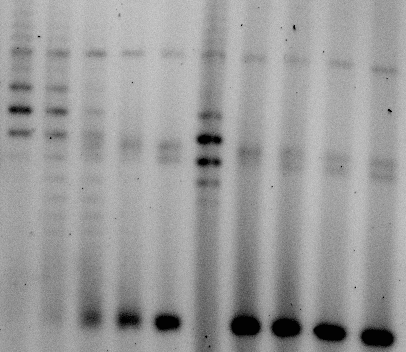
\includegraphics[width=\textwidth]{figures/diurnal/Y_CQ20_topoI_zoom_inv.png}
  \end{minipage}
  \begin{minipage}{.33\textwidth}
    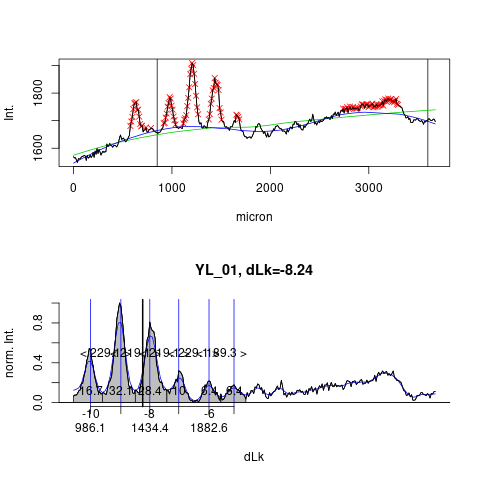
\includegraphics[width=\textwidth]{figures/diurnal/YL_01.png}
  \end{minipage}
  \begin{minipage}{.39\textwidth}
    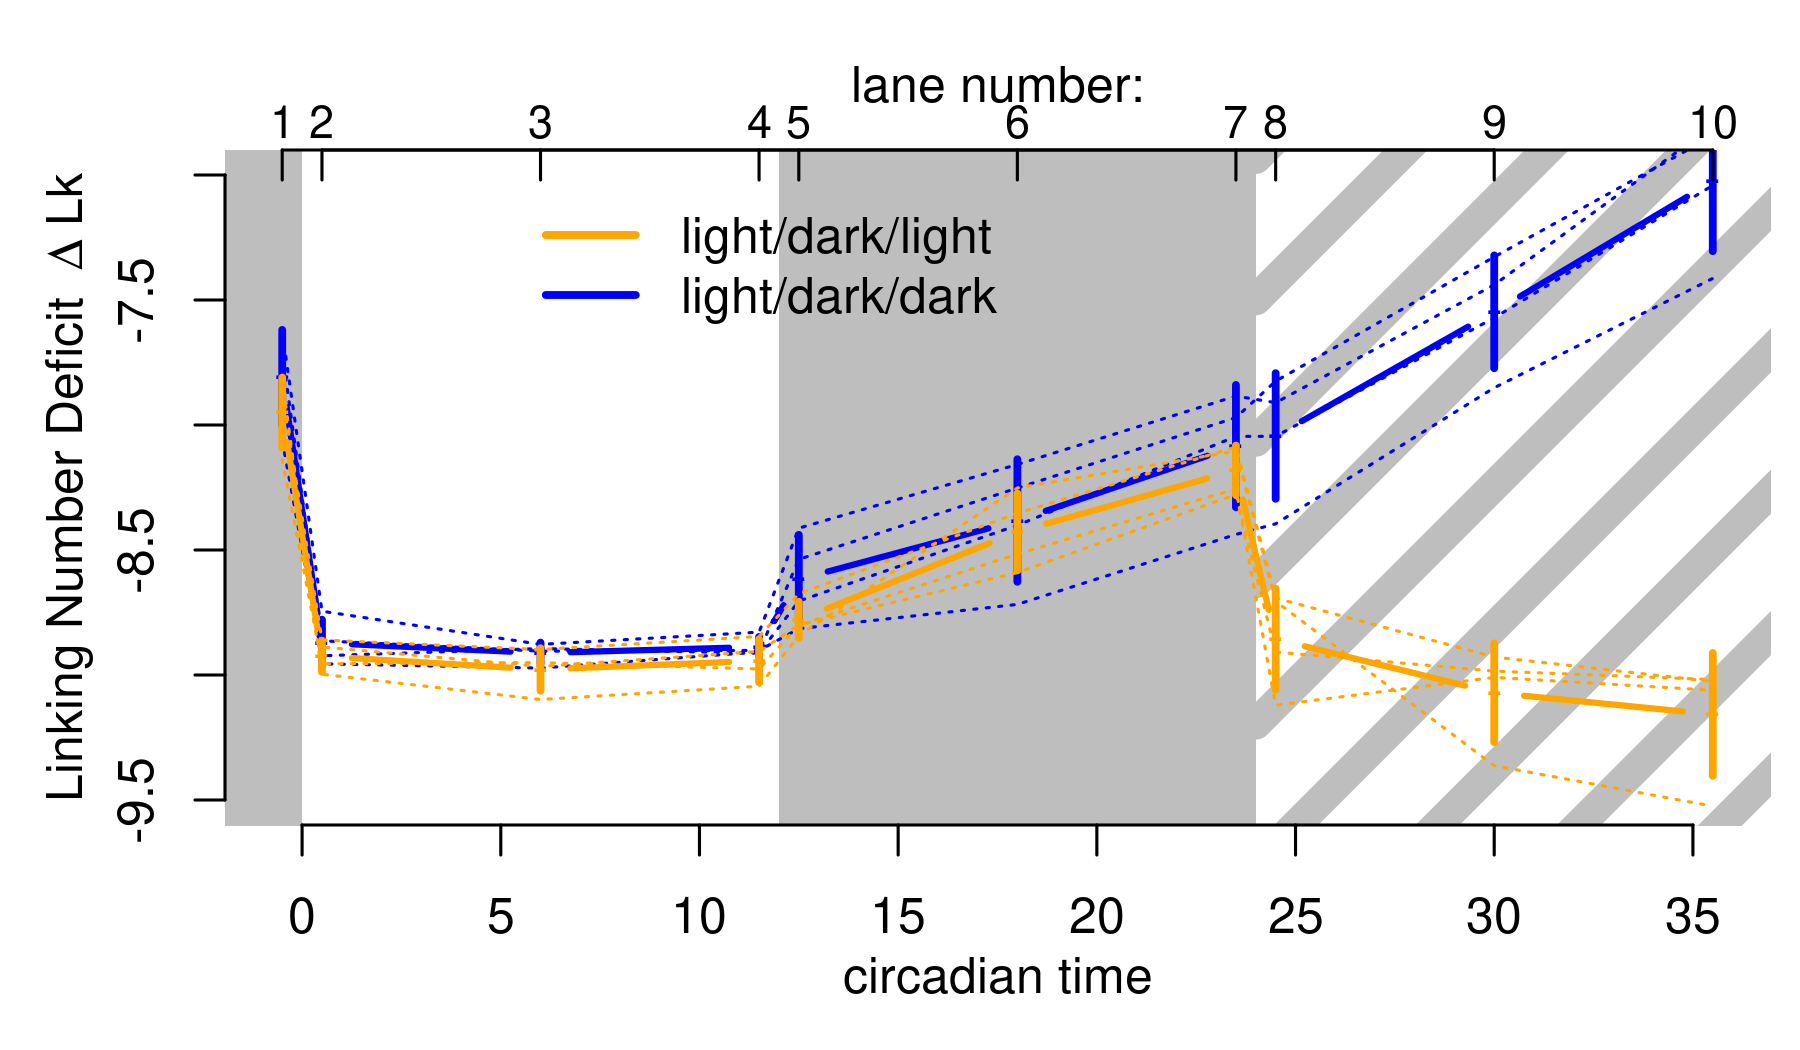
\includegraphics[width=\textwidth]{figures/diurnal/linkingNumbers.png}
  \end{minipage}
   
  \vspace{-.75cm}
  \textbf{A}\hspace{.26\textwidth}\textbf{B}\hspace{.33\textwidth}\textbf{C}
  \vspace{.25cm}
  
  \caption{\textbf{Chloroquine Gel Analysis: Calibration \& Diurnal
      Supercoiling}. \small{\textbf{A:} Mobility after relaxtion with
      topoisomerase I on an agaorse gel with \SI{20}{\ugml} CQ
      confirms the faster migration of fully relaxed plasmids at these
      conditions. Lanes 1-5: plasmids from pooled light phase samples
      (YL). Lanes 6-10: plasmids from pooled dark phase samples
      (YD). The topoisomerase I reaction was run for 1, 5, 10 and 30
      min at \SI{37}{\celsius} (lanes 2-5, 7-10). The samples in lanes
      1 and 6 were treated as the 30 min samples, but did not contain
      topoisomerase I. \textbf{B:} Quantification of the linking
      number deficit $\Delta Lk$ for lane 2 (YL, 1 min) from
      electropherograms of the gel in (E).  See Methods for details;
      in short: a baseline was determined in two steps (top panel) and
      subtracted from the signal. For the range that included all
      topoisomers of interest (vertical lines in top panel) the
      location of peaks (bottom panel: vertical blue lines and x-axis
      annotation) was detected from a smoothed version of the signal
      (blue line). All peaks were assigned consecutive integral
      linking number values $\Delta Lk$ with an estimated offset from
      the relaxed form with $Lk=0$. The areas under the peaks
      $A_{\Delta Lk}$ were calculated (gray areas) and the average
      linking number deficit of the sample was then determined as the
      center of mass $\Delta \overline{Lk} = \sum{(\Delta Lk \cdot
        A_{\Delta Lk})}/\sum{A_{\Delta Lk}}$ of all topoisomer bands
      (thick black horizontal line and top axis
      annotation). \textbf{C:} Diurnal time-series of the average
      linking number deficits ($\Delta \overline{Lk}$) of the
      pCA2.4\_M plasmids, calculated from three replicates of the gel
      in Figure \ref{fig:diurnalcq}A and one replicate of the gel in
      \ref{fig:diurnalcq}B.  The dotted thin lines are values from
      the 4 different gels and the thick lines are their means and
      standard deviations.  Gray background indicates the dark
      phases. One culture (blue line, light/dark/dark) did not receive
      the final 12 h of light and remained in the dark.  Note, that
      lower values indicate more \textbf{negative} supercoiling
      (higher $|\Delta \overline{Lk}|$).}}
  \label{fig:topoi} 
\end{figure}

   
\paragraph{Gradual Plasmid Relaxation in Dark Phase, Quick Supercoiling in
  Light.}  To clarify the unresolved issue whether DNA supercoiling is
higher during the light or dark phases, we first measured supercoiling
of endogenous plasmids of \textit{Synechocystis sp.} PCC6803 (Moscow
strain) \raim{and \textit{Synechococcus elongatus} PCC 7942} during
diurnal light/dark (12 h/12 h) conditions and a prolonged dark phase
(12 h light, followed by 24 h dark).  A large sample volume
(\SI{25}{\mL} was required to obtain enough plasmids, and direct
mixing of the sample with an equal volume of pre-cooled pure ethanol
was key to successful plasmid extraction. However, the yield was still
very low, limiting the amount of gels that can be run from one sample.

Multiple putative topoisomer bands were detected at all sampled time
points by agarose gel electrophoresis supplemented with chloroquine at
either \SI{1}{\ugml} (Fig. \ref{fig:diurnalcq}A) or \SI{20}{\ugml}
(Fig. \ref{fig:diurnalcq}B). \scyst{} contains three short
plasmids, two at 2.4 kb \cite{Yang1993b, Yang1994} and one at 5.2 kb
\cite{Xu1997b} . Restriction analysis and Southern blots confirmed
that the most pronounced topoisomer bands were obtained for plasmid
pCA2.4\_M (Fig. \ref{fig:diurnalcq}C \& D).

The migration distances on the gels were different between samples and
the relative differences reversed between the two CQ
concentrations. This change of relative migration speed indicates that
plasmids are still negatively supercoiled at the low, but positively
supercoiled at the high concentration. Plasmids which were originally
more relaxed migrate slower and faster at the low and high
concentrations, respectively.  Topo I relaxation time series of pooled
samples from light and dark phases further confirmed that more relaxed
plasmids migrate faster at the high CQ concentration
(Fig. \ref{fig:topoi}A).

Next, we quantified the agarose gels by generating electropherograms
of each lane in ImageJ. A baseline correction and peak detection and
peak area quantification were performed in R
(Fig. \ref{fig:topoi}B). For each sample an average linking
number deficit $\Delta \overline{Lk}$ was calculated and plotted as time series
over the light/dark cycles.  Plasmids were more supercoiled (higher
$|\Delta \overline{Lk}|$) during light phases, and reached a maximal level only
30 min after transition to the light phase. This level was maintained
or only slightly increased throughout the 12 h light phase.  During
the dark phase the transition was slower, and plasmids became
progressively more relaxed during the 12 h, and relaxation continued
at equal pace during an additional 12 h dark phase
(Fig. \ref{fig:topoi}C).

The maximal linking number differences between light and dark phase
were only $\Delta \Delta \overline{Lk} \approx 1$, and $\Delta \Delta
\overline{Lk} \approx 2$ after the prolonged dark phase.


\section{Discussion}

supercoiling of pCA is higher during the day, and lower during the
night, extended night relaxes plasmid even more, consistent
with the experiment by \cite{Woelfle2007} if interpreted
as we suggest

woelfle2007: wrong interpretation, likely also in synechococcus
supercoiling is decreased during the dark phase, esp. a prolonged
dark phase as shown in Fig XYZ of the publication,


vijayan09: corrected the intepretation of gels, but failed to mention
it!

\clearpage

\section{Materials and Methods}

\paragraph{pUC19 Plasmid Extraction.}
The vector DNA plasmid pUC19 (Roth: X911.1) was transferred into
\textit{Escherichia coli} DH5$\alpha$ via heat shock
transformation. DH5$\alpha$\_pUC19 was inoculated into LB medium and
grown overnight at \SI{37}{\celsius} and \SI{250}{rpm}. The preculture
was diluted 1:200 in fresh LB and grown for another \SI{3}{\hour}, and
harvested in exponential phase. The culture was centrifuged and pUC19
was isolated with ZymoPURE's Plasmid Maxiprep Kit. The isolated
plasmid was then purified (linear and open circular forms digested)
via T5 exonuclease (NEB: M0363) reaction and the NucleoSpin Gel and
PCR Clean-up kit (Machery-Nagel). The final plasmid DNA
concentration was determined with the Nanodrop.
%
\paragraph{pUC19 Relaxation Series.}
The pUC19 plasmid extract was split and \SI{1}{\ug} samples were
incubated with 0--3000 \si{\ugml} chloroquine in \SI{24}{\uL} of the
Cut Smart reaction buffer for \SI{15}{\min} at \SI{37}{\celsius}. Then
\SI{1}{\uL} (\SI{5}{U}) topoI (NEB: M0301) was added and the
samples incubated for another \SI{15}{\min} at the same
temperature. The reaction was stopped by incubation at
\SI{65}{\celsius} for \SI{20}{\min} and samples were purified with the
NucleoSpin Gel and PCR Clean-up kit (Machery-Nagel) to remove the
enzyme and the intercalator.

\paragraph{\scyst{} Strain and Culturing Conditions.}
Diurnal plasmid supercoiling time-series were established at
conditions and time-points identical to those used for the
transcriptome study in ref. \cite{Lehmann2013, Beck2014}.  The
glucose-tolerant and motile wild-type strain PCC-M of Synechocystis
sp. PCC 6803 (obtained from S.  Shestakov, Moscow State University,
Russia), was grown photoautotrophically in BG11-medium at
\SI{30}{\celsius} under continuous illumination with white light at
\SI{80}{\photons} (Versatile environmental test chamber; Sanyo) and
with a continuous stream of air in two airlift reactors (Schlenk
tubes) with 800 mL culture volume.  The optical density at 750 nm of
the culture was monitored (Specord200 Plus; Analytik Jena). Cultures
where then entrained to 12 h/12 h light/dark cycles for three
consecutive days and diluted to $\OD{}\approx 0.5$ one day before
sampling. Samples for plasmid analysis and \OD{} were then taken at
the indicated timepoints for 1.5 days. One culture was kept in dark
for the last 12 h of sampling.

\paragraph{Plasmid Extraction from \scyst{} Cultures.}
\SI{25}{\mL} of cell culture were mixed with \SI{25}{\mL} of
pre-cooled undenatured 95\% ethanol (\SI{-80}{\celsius} and on dry ice
during sampling), in \SI{50}{\mL} centrifuge tubes and stored at
\SI{-80}{\celsius} until processing. After thawing on ice, the
supernatant was discarded after centrifugation for \SI{10}{\minute} at
\SI{4}{\celsius} and \SI{4000}{g}. The QIAprep Spin miniprep kit was
used according to manufacturer's instruction, except for additional
enzymatic steps during lysis. The cell pellet was resuspended in
\SI{250}{\micro\liter} Qiagen P1 solution and transferred to
\SI{1.5}{\mL} reaction tubes. Then \SI{50}{\micro\liter} lysozyme 
solution (\SI{50}{\milli\gram\per\milli\liter}) was added, mixed, and
incubated for \SI{1}{\hour} at \SI{37}{\celsius}.  After the addition
of \SI{55}{\micro\liter} of \SI{20}{\percent} SDS and
\SI{3}{\micro\liter} of proteinase K
(\SI{20}{\milli\gram\per\milli\liter}), the reaction mixture was
incubated at \SI{37}{\celsius} for \SI{16}{\hour}.  Starting with the
alkaline lysis with the Qiagen P2 solution, all further steps
(QIAprep Spin Miniprep Kit) were carried out with
amounts that were adjusted to the initial volume. Next, the
concentrations and quality (260/280, 230/280 ratio) was determined
using the Nanodrop \todo{model} .  The PlasmidSafe enzyme mix (epicentre,
cat. no. E3101K) was used for removal of linear DNA according to the
manufacturer's protocol and incubated at \SI{37}{\celsius} for
\SI{30}{\minute} and purified with QIAprep spin columns using 5
volumes of the PB buffer. The final plasmid DNA concentration was
determined with the Nanodrop.


\paragraph{\scyst{} Plasmid Restriction and Relaxation Analyses.}
A pooled sample of plasmid extracts from \scyst{} was subjected to
rectriction by NcoI (Thermo Scientific: FD0573), which has a single
cut site in pCA2.4\_M but not in the similarly sized pCB2.4\_M.
\SI{1.5}{\uL} of FastDigest buffer and \SI{1}{\uL} of restriction
enzyme were added to \SI{12.5}{\uL} of plasmid samples. Reactions were
incubated for \SI{30}{\minute} at \SI{37}{\celsius} and stopped by
addition of \SI{3}{\uL} of 6x DNA loading dye with \SI{1}{\percent}
SDS and incubation at \SI{80}{\celsius} for \SI{15}{\minute}. The
resulting \SI{18}{\uL} were loaded directly onto the agaorse gel of
the time series in Figures \ref{fig:diurnalcq}A and C.

To test plasmid relaxation by topoisomerase I pooled samples from
light and dark phases were split and for each reaction \SI{10}{\uL} of
plasmid extracts were mixed with \SI{5}{\uL} 3x reaction buffer (150
mM Tris, 150 mM KCl, 30 mM MgCl2 , 1.5 mM DTT, 0.3 mM EDTA,
\SI{90}{\ugml} BSA) with or without 1 U of TopoI (Invitrogen,
Cat. no. 38042-024). The reactions were incubated at \SI{37}{\celsius}
and stopped after the indicated times by addition of \SI{3}{\uL} of 6x
DNA loading dye with \SI{1}{\percent} SDS at \SI{80}{\celsius} for
\SI{15}{\minute}. The resulting \SI{18}{\uL} were loaded onto the
agarose gel (Fig. \ref{fig:diurnalcq}E).

\paragraph{Chloroquine Agarose Gel Electrophoresis.}
Agarose gels with different concentrations of chloroquine diphosphate
(CQ) were used to determine the relative migration speed of
supercoiled topoisomers. 1.2\% agarose gels in 0.5x TBE were prepared
by heating to boiling. After cooling (hand-warm) CQ was added to the
indicated final concentration from a stock solution
(\SI{10}{\milli\gram\per\milli\liter}) and the mixture poured into the
gel chamber. The running buffer was 0.5x TBE buffer with the same CQ
concentration as the gel. For each sample, \SI{250}{\ng} plasmid DNA
was mixed with loading dye and filled up to \SI{30}{\uL} with water.
Gels were run for \SIrange{16}{24}{\hour} at \SI{40}{\volt}
(\SI{1.8}{\volt\per\cm}) in a Peqlab gel chamber, covered in foil to
protect from light. Gels were then washed two times for
\SI{30}{\minute} in \SI{250}{\mL} 0.5x TBE buffer to remove the CQ,
and stained with \SI{25}{\uL} Sybr Gold in \SI{225}{\mL} 0.5x TBE
buffer for \SIrange{3}{24}{\hour} and imaged on a BioRad Imaging
System (ChemiDoc MP). Washing and staining were also performed
light-protected.

\paragraph{Soutern Blots of Agarose Gels.}

Probes for Southern blots were generated by colony PCR using the
primers in Table \ref{tab:blot} (PCR programm: 3 min,
\SI{95}{\celsius}; 35x(\SI{95}{\celsius} 30s, \SI{50}{\celsius} 30s,
\SI{72}{\celsius} 1 min); \SI{72}{\celsius} 5 min).  The products were
isolated by cutting the band from an agarose gel and clean-up with the
NucleoSpin Extract II kit (Macherey-Nagel).  Labelled DNA was
generated using the same PCR program with the DIG Easy Hyb (Roche, 1603558)
mix, according to manufacturer's instruction.
%
Soutern blots were generated using the CDP-Star kit with slight
modifications as follows.  Gels were blotted onto a nitrocellulose
membrane using a vacuum blotter \todo{model?} (\SI{90}{\min} with
\SIrange{5}{7}{mm Hg}, in 10x SSC buffer). The membrane was
pre-hybridized for \SI{1}{\hour} at \SI{50}{\celsius}.  The probes
were denatured (\SI{95}{\celsius}, \SI{15}{\min}) and cooled on ice,
then transfered to the blot and hybridized over night at
\SI{50}{\celsius}. The membran was washed 2x \SI{5}{\min} mit 2x SSC,
0.1 \% SDS at \SI{50}{\celsius}, then with 2x 15 min mit 0.1x SSC und
0.1 \% SDS at \SI{65}{\celsius}, and cross-linked with UV light
\todo{model} for \SI{10}{\min}. All further steps were performed
according to the CDP-Star manual and \raim{blots were imaged on a
  BioRad Imaging System (ChemiDoc MP).}

%Ich vermute, dass die Gele mit Dem Vakuum-Blotter geblottet wurden (mein Standard-Protokoll sagt, dass 90 min bei 5-7 mm Hg Unterdruck mit 10x SSC-Puffer geblottet wird). Danach wird die Membran zweimal mit 2x SSC-Puffer gewaschen und dann 5-10 min mit UV gecrosslinkt. Der Rest müsste so passen.




\begin{table}[ht!]
  \begin{tabular}{c|c|l}
    Plasmid & Direction & Sequence \\
    \hline
    pCA2.4\_M &forward & ACAGGGGTAAATGAGTGCCG\\ % grep-confirmed
    &reverse & GCAAGCAGTCCTCCACAAGA  % grep-confirmed, revcomp
  \end{tabular}
  \caption{\textbf{Southern Blot Probes: Primer Sequences.}}
  \label{tab:blot}
\end{table}


\paragraph{Analysis of Gel Electropherograms.}
Electropherograms were extracted in ImageJ for each lane and analyzed
in R, using LOESS smoothing and peak detection functions from the
\texttt{msProcess} R package (version 1.0.7)
(\url{https://cran.r-project.org/web/packages/msProcess/}). A baseline
was determined in two steps using the \texttt{msSmoothLoess} function
(Fig. \ref{fig:diurnalcq}F, top panel).  The first step used the full
signal and served to determine the coarse positions of peaks.  The
final baseline was then calculated from the signal after removal of
peak values. This baseline was subtracted from the total signal to
detect peaks (bands) with the \texttt{msPeakSimple} function from
\texttt{msProcess} and calculate peak areas.  For the total RNA
analysis, the baseline signal stems from mRNA and rRNA degradation
fragments, and was used to calculate ratios of rRNA peak areas to the
``baseline'' area.

\paragraph{Calculation of $\Delta Lk$.}
For the diurnal time series we quantified relative linking number
deficits (Fig. \ref{fig:diurnalcq}F, bottom panel) by analysis of
topoisomer peak areas.  Peaks were assigned consecutive
integral linking number values $\Delta Lk$ with an estimated offset of
a reference peak from the relaxed form with $Lk=0$. The areas under
the peaks $A_{\Delta Lk}$ were calculated and the average linking
number deficit of a sample was then determined as the center of mass
\begin{equation}
  \label{eq:dlk}
  \Delta \overline{Lk} = \sum{(\Delta Lk \cdot
    A_{\Delta Lk})}/\sum{A_{\Delta Lk}}
\end{equation}
of all topoisomer bands.

Note, that the true $\Delta Lk$ of bands from the relaxed plasmid was
not determined, eg. by Keller's band counting method
\cite{Keller1975b}.  The calculated $\Delta Lk$ values refer to an
arbitrary assignment of a reference band that was present in most
lanes to $\Delta Lk=-8$, and this can be considered a maximal estimate
of the true $\Delta Lk$ based on the distance of topoisomer and
relaxed DNA bands in the topoisomerase I relaxation experiment in
Figure \ref{fig:diurnalcq}G.

\bibliographystyle{plain}
%% SWITCH between global and local/git bibtex file
%% and use `bibexport -o cqgels.bib cqgels.aux` to update local
% citations for goi.tex
%\bibliography{/home/raim/ref/tata}
\bibliography{cqgels}

\end{document}
